\documentclass[whitelogo]{tudelft-report}

%% Packages
\usepackage{natbib}
\usepackage{changes}
\usepackage{tabu}
\usepackage{booktabs} %for horizontal lines in tables: \toprule[1pt], \midrule[1pt], \bottomrule[1pt]

%% Layout: customized for this certain report
\setlength{\parindent}{0cm} %no indentation in first line of paragraph

%% Compilation: to compile the pdf do (if it is not done automatically):
%% xelatex report
%% bibtex report
%% xelatex report
%% xelatex report


\begin{document}

%% Use Roman numerals for the page numbers of the title pages and table of
%% contents.
\frontmatter

%% Uncomment following 19 lines for a cover with a picture on the lower half only
%\title[tudelft-white]{Title}
%\subtitle[tudelft-cyan]{Optional subtitle}
%\author[tudelft-white]{J.\ Random Author}
%\affiliation{Technische Universiteit Delft}
%\coverimage{cover.jpg}
%\titleoffsetx{10cm}
%\titleoffsety{10cm}
%\afiloffsetx{1cm}
%\afiloffsety{18cm}
%\covertext[tudelft-white]{
%    \textbf{Cover Text} \\
%    possibly \\
%    spanning 
%    multiple 
%    lines
%    \vfill
%    ISBN 000-00-0000-000-0
%}
%\makecover

%% Uncomment following 16 lines for a cover with a picture on the lower half only
\title[tudelft-white]{CIE5308}
\subtitle[tudelft-black]{Breakwater Rehabilitation Romano Port}
\author[tudelft-white]{{J. Gundlach} -- {C. Rozas} -- {L. Lange}}
\affiliation{Delft University of Technology}
\coverimage{title.jpg}
\covertext[tudelft-white]{
    \textbf{Group 3} \\
    %possibly \\
    %spanning 
    %multiple 
    %lines
    \vfill
}
\setpagecolor{tudelft-cyan}
\makecover[split]


%% Include an optional title page.
\begin{titlepage}


\begin{center}

%% Insert the TU Delft logo at the bottom of the page.

%% Print the title in cyan.
{\makeatletter
\largetitlestyle\fontsize{64}{94}\selectfont\@title
%\largetitlestyle\color{tudelft-cyan}\Huge\@title
\makeatother}

%% Print the optional subtitle in black.
{\makeatletter
\ifx\@subtitle\undefined\else
    \bigskip
   {\tudsffamily\fontsize{22}{32}\selectfont\@subtitle}    
    %\titlefont\titleshape\LARGE\@subtitle
\fi
\makeatother}

\bigskip
\bigskip

by
%door

\bigskip
\bigskip

%% Print the name of the author.
{\makeatletter
%\largetitlefont\Large\bfseries\@author
\titlestyle\fontsize{10}{10}\selectfont\@author
\makeatother}

\bigskip
\bigskip

% to obtain the degree of Master of Science
% %ter verkrijging van de graad van Master of Science
% 
% at the Delft University of Technology,
% %aan de Technische Universiteit Delft,
% 
% to be defended publicly on Tuesday January 1, 2013 at 10:00 AM.
% %in het openbaar de verdedigen op dinsdag 1 januari om 10:00 uur.

\vfill

\begin{tabular}{lll}
    Student numbers: & 4450426 -- 4519388 -- 4512022 \\
    Project duration: & \multicolumn{2}{l}{March 17, 2016 -- April 1, 2016} \\
%     Thesis committee: & Prof.\ dr.\ ir.\ J.\ Doe, & TU Delft, supervisor \\
%         & Dr.\ E.\ L.\ Brown, & TU Delft \\
%         & Ir.\ A.\ Aaronson, & Acme Corporation
\end{tabular}
%% Only include the following lines if confidentiality is applicable.

% \bigskip
% \bigskip
% \emph{This thesis is confidential and cannot be made public until December 31, 2013.}
% %\emph{Op dit verslag is geheimhouding van toepassing tot en met 31 december 2013.}

% \bigskip
% \bigskip
% An electronic version of this thesis is available at \url{http://repository.tudelft.nl/}.
% %\\[1cm]

%\centering{
\includegraphics{cover/logo_black}}


\end{center}

\begin{tikzpicture}[remember picture, overlay]
    \node at (current page.south)[anchor=south,inner sep=0pt]{
        
\includegraphics{cover/logo_black}
    };
\end{tikzpicture}

\end{titlepage}



% \chapter*{Preface}
\setheader{Preface}

Preface\ldots

\begin{flushright}
{\makeatletter\itshape
    \@author \\
    Delft, January 2013
\makeatother}
\end{flushright}



\tableofcontents

%% Use Arabic numerals for the page numbers of the chapters.
\mainmatter

%\chapter{Notes}

\section{18.03.16 - lecture introducing exercise}

\textbf{Main aim}: design breakwater
\begin{enumerate}
 \item new breakwater
 \item adjust existing one
\end{enumerate}

\textbf{Location}:
\begin{itemize}
 \item ..
\end{itemize}

\textbf{Present situation}:
\begin{itemize}
 \item cross-section, what they were supposed to build
 \item slide 9: measured cross-section
\end{itemize}

\textbf{Assignment}:
\begin{itemize}
 \item three locations
 \item three design lifes: after so many years needs to be maintained/rebuild, not for design cinditions!
 \item something with the existing (Bas)...?
\end{itemize}

\textbf{Design}:
\begin{itemize}
 \item assume: subsoil no problem
 \item Any idea where the rock comes from? Quarries in ALbania? Albania exports a lot of Marble to Italy. How about the stones sorted out?
 \item Infra structure in Albania not as good.
 \item Google Earth because you can check time. Check -design period and +design period from present.
 \item Play with colors in picture editor. Image processing for bathymetry stuff.
 \item Map Room: Libarary of faculty of architecture, first floor within library. And webpage of this library? And webapp.navionics.com (not working for 4G.
 \item Check wave data from design wind speed $\rightarrow$ should be in same magnitude as from Argoss (verify data)
\end{itemize}

\textbf{Argoss}:
\begin{itemize}
 \item sells  wave data
 \item www.waveclimate.com
 \item TuDelft DuT4321 valid until 31.3.
 \item Size of piece: find balance (density of data is the same, too big, not appropriate anymore, too small, not enough data any more)
 \item 1D, 2D, 3D
 \item don't use their model for nearshore
\end{itemize}

\textbf{B.C.}:
\begin{itemize}
 \item B.C. damage vs. B.C. operation of port
 \item 
\end{itemize}

\textbf{Presentation}:
\begin{itemize}
 \item Why did you make this choices you made?
 \item Presentation and questions of group will be graded.
 \item No obvious information in the presentation
 \item 
\end{itemize}

\textbf{Report}:
\begin{itemize}
 \item Indicate 2.1 to 2.6 clearly in report
 \item Make it possible to enable contractor for a pricing
 \item Drawing on A3
 \item only cross-section, only one
 \item head needs not to be designed?
 \item only 10 pages text
 \item report should be understandable without annex
 \item 
\end{itemize}

\textbf{Calculation}:
\begin{itemize}
 \item bonus for differences due classical and probabilistic approach
 \item No assessment on skills in maths
 \item 
\end{itemize}

\textbf{PIANC}:
\begin{itemize}
 \item kennisbank waterbouw
 \item ''codes, standards and design guides``
 \item ...
 \item ''Books and reports``
\end{itemize}


\textbf{Check}:
\begin{enumerate}
 \item google earth
 \item make pdfs from ppt's
 \item Argoss book online or from library
 \item check demands on slides, slide 21  e.g.
 \item 
\end{enumerate}



\chapter{Introduction}

\section{General Task}

By \textit{Group 3} the breakwater in the South is looked at:
\begin{itemize}
 \item adjacent to roundhead, axis 315\textsuperscript{o}
 \item rubble mound single layer cubes
 \item rehabilitation
 \item 100 years design life
 \item quay wall in future
\end{itemize}

\citep{Geim2001} $\leftarrow$ this can be deleted as soon, as there is any other citation we can place, so to prevent error messages due to ``no citations found''
\chapter{Design Criteria}

see exercise 3.1

\begin{center}
\begin{table}[!htb]
\begin{tabu}{X[2l] X[1c] X[2c] X[1c] X[1c]}
\textbf{Requirement} & \textbf{Return period} & \textbf{Verification method(s)} & \textbf{Design value} & \textbf{Calculated value}\\
\\
\toprule[2pt]
this is supposed to be a verly long text to check whether it will automatically insert a line break & this is supposed to be a verly long text to check whether it will automatically insert a line break & this is supposed to be a verly long text to check whether it will automatically insert a line break & this is supposed to be a verly long text to check whether it will automatically insert a line break & this is supposed to be a verly long text to check whether it will automatically insert a line break\\
\\
× & × & × & × & ×\\
\\
× & × & × & × & ×\\
\\
× & × & × & × & ×\\
\\
× & × & × & × & ×\\
\\
× & × & × & × & ×\\
\\
× & × & × & × & ×\\
\\
× & × & × & × & ×\\
\\
× & × & × & × & ×\\
\\
× & × & × & × & ×\\
\bottomrule[2pt]
\end{tabu}
\caption{List of requirements}
\label{tab:requirements}
\end{table}
\end{center}

\chapter{Boundary Conditions}

see exercise 3.2

\section{Location}
The Romano Port is located at the west-coast of Albania in the Adriatic Sea, 7.5 km north from the city Durr\"{o}es and around 30 km from the capital of Albania Tirana. 
Albania has a HDI (Human Development Index) of 7.33 which puts the country to the "high human development category" according to the HDI report of the UN 2015 like Algeria, Brazil or Turkey. 

\section{Subsoil}
Subsoil matters are not included in this breakwater design. It is assumed, that the soil can resist all loads and that no soil-improvement needs to be done.
\section{Reference levels}
\begin{center}
\begin{table}[!htb]
\begin{tabu}{X[2l] X[2c]}
\toprule[2pt]
\textbf{Tide} & \textbf{Water Level [m AL]} \\
\\
\midrule
HAT & -0.324\\
\\
HHWS & -0.336\\
\\
MHWS & -0.349\\
\\
MHW & -0.421 \\
\\
MHWN & -0.476\\
\\
MLWN & -0.605\\
\\
MLW & -0.652\\
\\
MLWS & -0.7\\
\\
LLWS & -0.71\\
\\
LAT & -0.722\\

\bottomrule[2pt]
\end{tabu}
\caption{Tidal water levels at Durr\"{o}es}
\label{tab:tidal_level}
\end{table}
\end{center}
As shown in table \ref{tab:tidal_level} the relative Albanian Level (AL) ,which is +0.535 m above Mean Sea Level, leads to the rewriting of tidal elevations. Every water level in this assignment will be given according to AL.

\section{Bathymetry}

\section{Additional Water Level}
Due to the following factors the water level rises for the design conditions with 1.3 m according to the mean water level:
\begin{itemize}
\item Tidal differenz: +0.211
\item Sea Level Rise: $0.005 m/year * 100 years = +0.5 m$
\item Seasonal effects: +0.07
\item Atmospheric pressure drop: +0.33 m
\item Wind set-up + seiches: +0.17	
\end{itemize}
Which leads to an increase of the water level in a hundred years for the combination of all effects of 1.281 m which will be considered as 1.3 m to get some small extra safety as an engineering approach.
\section{Waves}
Wave heights and the return period of wave events are essential for determine the dimensions of a breakwater. Especially for estimating the size of the amour layer and hence the size of under-layer material, is the wave hight the dominant parameter. Furthermore the order of the run-up and over-topping magnitude is mainly dependent on the wave hight.
\subsection{Design storm}
The design storm with less than 20\% probability of failure of the breakwater within a lifetime of 100 years returns every 500 years.
The available 22 years of (modelled) wave data\footnote{ARGOSS XX} close to the site is analysed in a Peak over Threshold analysis using a threshold of $H_s=1.5m$, a storm duration of nine hours and a Weibull distribution to extrapolate the data. The wave-data from Argoss were checked for reliability (see appendix).
This yields a significant wave height of $H_{ss}=7.91m$ for a 500 year storm, which is chosen to be the deep water design wave height: $H_{ss,d}=7.91m$.

According to the distribution of the wave hight over peak wave periods from the wave model of Argoss %(appendix \ref{Distribution_pperiod}) 
the peak period was chosen to be 11 seconds.
The Distribution of the wind and the wind speed at 10 m hight was created through the Argoss data set too and shows velocities up to 20 m/s with varying directions
%\ref{Windrose}
. The main  directions are NW, N, NE, SSE and S but for the model just NW and S winds are considered with 20 m/s because of the influence at the breakwater as a worst case scenario.

\subsection{Near-shore Wave model}
SwanOne was used to estimate the wave development at near-shore. The Input parameters are in this case:
\begin{itemize}
\item The generated two dimensional bathymetry
\item The additional water level
\item The wave hight
\item Peak period
\item Wind velocity
\item Angle of incidence 	
\end{itemize}

\begin{figure}[H]
\center
\fbox{
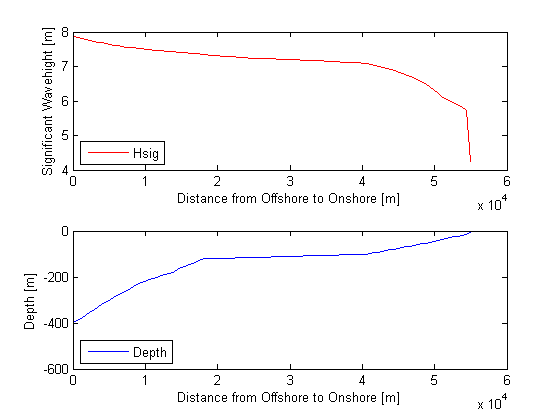
\includegraphics[width=\textwidth]{images/Hsig_Depth_Plot.png} 
}
\caption{Rose-diagram waves}
\label{Hsig_Depth_Plot}
\end{figure}
In the Swan model additional wind was  included but the set-up due to wave action was neglected, because it is included in the offshore wave data we gained and currents were neglected due to the location in the Mediterranean See with hardly any currents.
Bathymetry,additional water level, wave hight, wind velocity and peak period were determined before, but now different angles of wave attack need to be considered.
For determine which angles are of interest for the occurrence of sea and swell waves the Argoss data are checked again 
%\ref{wavedata_angle}
. As a result from the analysis the dominant direction for waves to occur are NW and S, which matches with the geographical expectations. Due to the orientation of the breakwater at the coast the waves from NW will arrive with a very large angle close to 90$^\circ$ according to the breakwater why the wave energy attacking the breakwater is quite small. Because of the small fetch length just wave with relative low energy will arrive perpendicular to the breakwater. The biggest influence is expected to come from the south and thus the angle of the waves to attack the breakwater will be around 45$^\circ$ which is the value used for the modulation in SwanOne. 
The model was simulating with a grid size of around 5.55 m per cell and 10,000 time steps per simulation to get an accurate result.
The final Simulation is shown in figure \ref{Hsig_Depth_Plot} and the actual value for the significant design wave hight from a one in 500 years storm at the near-shore in a depth of 12 meter is 5.614 m.
\chapter{Design Calculations}

\section{Armour Layer}
For this group it is stated to build a breakwater with an armour layer of cubes. To calculate the cube size and weight of this armour layer the Van der Meer equation (1988) on the website cress\footnote{http://www.cress.nl/Regel.aspx} will be used. The input values, the equation and the damage categories can be found in the appendix under Design Armour Layer \ref{tab:design_armour}. Basically there are two material for cubes: Concrete and Rock. But due to the dimensions and the limited availability of big size rocks the cubes need to be made of concrete. The result of the calculation with Cress for the concrete cubes gives a Dn of 2.14 meter and a weight of 25 tonnes.
\section{Toe}

\section{Overtopping}

\section{Run-Up}

\section{Wave Transmission}

\section{Future Quay Wall}
The design has to take into account the presence of a future quay wall.
This puts requirements on the space available behind the breakwater and the design of the landward side of the breakwater, in such a way, that it does not hinder the future construction of a quay wall.
Especially due to the space requirement a vertical wall would be the best option in terms of the future quay wall (for instance to place a quay wall on piles, put sheetpiles and backfill them etc.).
Using a caisson or a concrete wall at the backside of the breakwater might be as costly as any other option, but more severe damage is expected due to an earthquake, which counteracts the demand for a 100 years lifetime and a minimum of maintenance, so these options are not considered further.

\chapter{Drawing}

see exercise 3.4


\clearpage
This is one single page, where we can add the folded A3 of our drawing after printing.
Included to not interrupt counting of pages.
\newpage
\chapter{Construction Method and Planning}

see exercise 3.5
\chapter{Further Research and Validation}

see exercise 3.6


%% Use letters for the chapter numbers of the appendices.
\appendix

\chapter{Function GumbelUnc.mat}


\begin{figure}[H]
\center
\fbox{
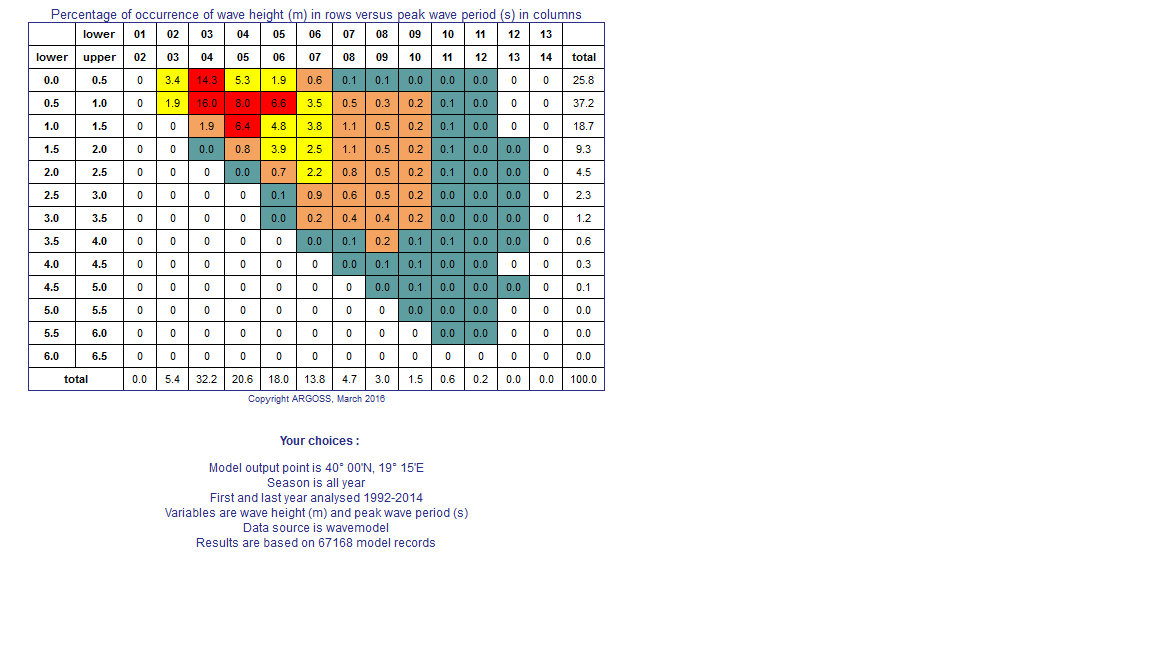
\includegraphics[width=\textwidth]{images/wave_pperiod_allyear.png} 
}
\caption[Distribution of peak-period over wave hight]{Distribution of peak-period over wave hight}
%\label{Distribution_pperiod}
\end{figure}


\begin{figure}[H]
\center
\fbox{
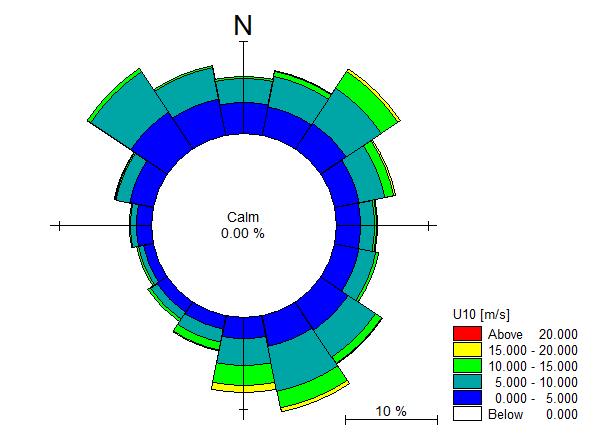
\includegraphics[width=\textwidth]{images/Rose_plot_u10.png} 
}
\caption[Rose-diagram with the distribution of the wind}
%\label{Windrose}
\end{figure}


\begin{figure}[H]
\center
\fbox{
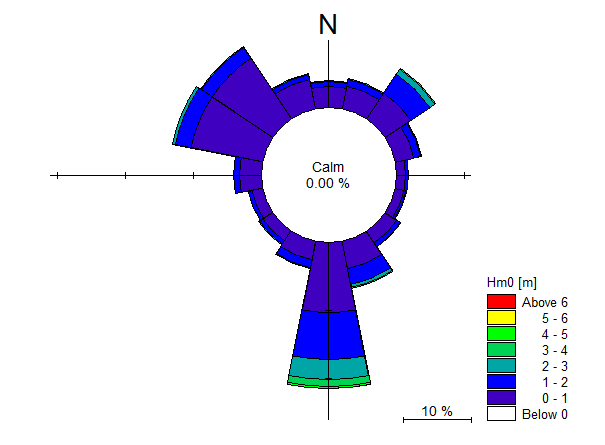
\includegraphics[width=\textwidth]{images/Rose_plot_Hoverall.png} 
}
\caption[Rose-diagram with the distribution of the waves}
%\label{wavedata_angle}
\end{figure}
Whatever XX


\bibliography{report}

\end{document}

